\chapter{Introduzione all'approccio SPICE}
	
	A livello accademico è stato descritto il principio di funzionamento dei \textit{MOSFET}, ossia dei transistor che utilizzano l'effetto di carico che si instaura tra uno substrato semiconduttivo e un metallo ossidato per movimentare delle cariche elettriche. In base al drogaggio dei terminali di \textit{source} e \textit{drain}, complementare a quello di \textit{bulk}, è possibile suddividere i transitori in due famiglie: gli \textit{n-MOS} (drogaggio di tipo $n$) e i \textit{p-MOS} (drogaggio di tipo $p$). In particolare la relazione statica che lega la corrente che scorre tra i terminali di drain e source è funzione sia della differenza di tensione $V_{gs}$ tra \textit{gate} e source, ma anche alla differenza di tensione $\Vds$ tra drain e source:
	\begin{equation} \label{eq:relstatica}
		I = K_n \frac W L \left[ \big(\Vgs - \Vtn\big)\Vds - \frac{\Vds^2}{2} \right]
	\end{equation} 
	In questa relazione è possibile osservare la presenza di 3 parametri fondamentali a determinare il comportamento del transistor: la \textit{conducibilità intrinseca} $K_n$, proprietà caratteristica del semiconduttore utilizzato per il bulk, e le dimensioni caratteristiche $W$ (larghezza) e $L$ (lunghezza) del canale conduttivo. Nella caratteristica statica fondamentale è anche la \textit{tensione di soglia} $\Vtn$ dipendente sia dalla costituzione del transistor, sia dalla differenza di tensione $V_{bs}$ tra bulk e source. 
	
	Il modello presentato in equazione \ref{eq:relstatica} è in realtà una versione approssimata della caratteristica di trasferimento reale di un transistor MOS e trascura molti fenomeni elettro-magnetici che nella realtà dovrebbero essere considerati; esso può essere utile a livello didattico per concepire il funzionamento di alcuni circuiti semplici, tuttavia per problemi più complessi un approccio analitico approssimato può portare a risultati fuorvianti. \\
	Un approccio simulativo è infatti più indicato per poter analizzare le prestazioni di circuiti più complessi in quanto a prova di errori (una volta che ci si è assicurati di aver implementato correttamente gli schematici) e permette di considerare effetti elettro-magnetici che analiticamente sarebbe difficile da studiare.
	
	\vspace{3mm}
	
	In ambito elettronico per effettuare delle simulazioni numeriche di circuiti si utilizzano i software cosiddetti \textit{SPICE} (acronimo di \textit{Simulation Program with Integrated Circuit Emphasis}); in particolare tra le numerose soluzioni disponibili sul mercato nel proseguimento del seguente testo verrà utilizzato il software gratuito \texttt{XScheme} \cite{xschem} per la realizzazione degli schematici che verranno simulati tramite l'applicativo \texttt{ngspice} \cite{ngspice}.
	
\section{Parametri di simulazione}
	Per poter effettuare delle simulazioni è necessario fornire al software una raccolta con le informazioni da utilizzare per modellare il transistor, ossia è necessario specificare tutti i parametri che possono essere sia geometrici, ma anche legati alle proprietà dei materiali. 
	
	Facendo diretto riferimento ai parametri presenti nell'equazione \ref{eq:relstatica} per un transistor è necessario in primo luogo indicare la conducibilità intrinseca \texttt{Kp} $[A/V^2]$, la lunghezza \texttt{L} $[m]$  e la larghezza \texttt{W} $[m]$  del canale conduttivo. Altri parametri geometrici che possono essere utilizzati per migliorare l'analisi è indicare sia perimetro che area per il terminale di drain (parametri \texttt{PD} $[m]$ e \texttt{AD} $[m^2]$) e il terminale source (parametri \texttt{PS} e \texttt{AS}).
	
	Come parametri funzionali per il calcolo della caratteristica statica dei MOSFET si menziona la tensione di soglia, modellata tramite il parametro \texttt{Vto} $[V]$. L'effetto body, dovuto alla differenza di tensione tra bulk e source, richiede invece di specificare il relativo coefficiente \texttt{Gamma} $\left[V^{0.5}\right]$ e il coefficiente superficiale \texttt{Phi} $[V]$. Come ultimo parametro di un transistor si menziona il coefficiente di modulazione di lunghezza di canale \texttt{Lambda} $\left[V^{-1}\right]$.
	
	\begin{table}[bht]
		
		\centering
		\begin{tabular}{ c c | p{2cm}  p{2cm}}
			& & \multicolumn{2}{c}{famiglia di transistor }  \\
			parametro & unità & n-MOS & p-MOS \\ \hline 
			\texttt{K} & $[A/V^2]$ & $50\cdot 10^{-6}$ & $20\cdot 10^{-6}$ \\
			\texttt{W} & $[m]$ & $50\cdot 10^{-6}$ & $20\cdot 10^{-6}$ \\
			\texttt{L} & $[m]$ & $50\cdot 10^{-6}$ & $20\cdot 10^{-6}$ \\
		\end{tabular}
		\caption{parametri di simulazioni utilizzati nel seguente documenti; i dati sono basati su transistor \textbf{ALTRE INFORMAZIONI}}
		
		
	\end{table}


	Un componente reale, in condizioni sia statiche, presenta delle perdite di corrente sia tra drain e source, sia tra gate e source, nel cosiddetto fenomeno della \textit{current leakage} (perdita di corrente) associato alle correnti parassite. Analizzando invece il comportamento dinamico del circuito è possibile osservare che i MOSFET presentano un'inerzia alla trasmissione di carica (rispetto ad ogni coppia di terminali): tali effetti di \textit{capacità parassite} possono essere modellate tramite l'inserimento nello schematico di capacità equivalenti. \\
	Nella pratica le relazioni che determinano correnti e capacità parassite sono complesse (equazioni fortemente non lineari) e dipendenti da molti parametri dei transistor stessi: non esiste dunque un modello univoco che può essere utilizzato per la simulazione dei circuiti (ad un livello di complessità simil-realistico), ma in generale ogni produttore mette a disposizione dei progettisti i loro modelli spice che possono dunque essere inclusi negli schematici per effettuare delle simulazioni più interessanti.
	
\section{\textit{Process Design Kit}: skywater}
	
	Il \textit{Process Design Kit}, spesso abbreviato dall'acronimo \textit{PDK}, è una suite di librerie e applicativi che permettono una progettazione corretta di un circuito integrato. In questi kit sono contenuti infatti tutti i modelli spice (sia dal modello lineare più semplice, sia a modelli del $4^\circ$ ordine più complessi) che possono essere utilizzati per le simulazioni, oltre che a una serie di informazioni che vincolano la progettazione per permettere di ottenere un prodotto che sia effettivamente utilizzabile nel mondo reale. Per esempio, oltre a tutte le informazioni riguardanti ingombri fisici, i PDK contengono le proprietà per simulare con maggior precisione le correnti e capacità parassite che si generano nel prodotto finito.
	
	\skywater, come dice il nome stesso, è dunque un PDK rilasciato pubblicamente frutto della collaborazione di Google con la fondazione Skywater; questo progetto, per come riportato dal team di sviluppo del PDK stesso, è ancora in fase sperimentale e dunque può non essere perfettamente accurato, tuttavia si osserva che lo stesso progetto deriva direttamente da PDK utilizzati da anni a livello professionale. \\
	L'idea alla base di questo progetto open source è quella di permettere a tutte le persone di progettare e prototipare circuiti integrati, permettendo la realizzazione pratica sfruttando il processo produttivo a $130 nm$ fornito da \texttt{SkyWater Technology foundry} \cite{fossi}.
	
	
	Sfruttando la suite di software composta da \texttt{XSchem}, \texttt{ngspice} e \texttt{skywater PDK} è possibile realizzare degli schematici e dei circuiti che si avvicinano il più possibile a dei circuiti reali.
	
	\subsection*{Contenuti del PDK}
		La libreria skywater mette a disposizione sostanzialmente 2 categorie di modelli spice per la simulazione:
		\begin{itemize}
			\item le \textit{primitive cells}, abbreviate PR, ossia i modelli associati ai mosfet (sia a 4 pin, sia a 3 pin con bulk collegato a massa), ma anche per altri componenti passivi che possono essere integrati su chip quali svariati tipi di resistenze (in funzione della potenza dissipabile), di capacità MIM (\textit{metal-insulator-metal}), diodi e diodi varicap;
			
			\item la \textit{digital standard cells}, abbreviate SC, sono invece già dei circuiti combinatori che sfruttano l'interconnessione delle celle primitive per realizzare porte logiche (and, or, not...) e altri circuiti combinatori (latch).
		\end{itemize}
		
		Nella libreria sono presenti diverse varianti di transistori caratterizzati sia principalmente dalle differenze di tensioni ammissibili tra le coppie di terminali dei componenti (si trovano componenti che funzionano per tensioni $\Vgs,\Vds$ di valori $1.8V,\ 3.3V,\ 5.0V, \ 20V$).  Leggendo la documentazione \cite{specsky} rilasciata dagli sviluppatori è inoltre possibile individuare i valori di lunghezza $L$ e larghezza $W$ ammissibili per la produzione di ogni tipo di mosfet.	
		
		La libreria delle standard cells derivanti dalle celle primitive sono divise in diverse famiglie caratterizzate dagli appellativi:
		\begin{itemize}
			\item \textit{high density} (HD) e \textit{high density low leakage} (HDLL), ossia porte logiche la cui caratteristica è di avere ingombri su chip più bassi (pari a $0.46\times 2.72 \mu m$) in modo da aumentare la densità di integrazione su scheda; la seconda tipologia, come si evince dal nome, è caratterizzata inoltra da una bassa dispersione di corrente elettrica. La tensione di alimentazione è posta a $1.8V$;
			\item le celle a bassa tensione (alimentazione $<2.0V$) sono classificate in base alla velocità di commutazione dei gate secondo gli appellativi \textit{low speed} (LS), \textit{medium speed} (MS) e \textit{high speed} (HS); in questa categoria è possibile rilevare anche le celle a basso consumo di potenza (categoria \textit{low power} LP). L'ingombro su scheda di queste celle elementari è pari a $0.48\times 3.33\mu m$;
			\item \textit{high voltage} (HVL) sono invece delle celle con tensione di alimentazione pari a $5.0V$ con ingombro su scheda di $0.48\times 4.07 \mu m$.
		\end{itemize}
	
		\paragraph{Corner spice models} La descrizione tramite un modello matematico astratto per predire il comportamento empirico di un componente analogico non sempre risulta essere accurato per via dei parametri di influenza esterni che il calcolatore non può considerare (come correnti e capacità parassite che si instaurano inevitabilmente tra i componenti).
		
		Per poter effettuare delle valutazioni più pratiche dei circuiti progettati, il pdk fornisce al progettista i cosiddetti modelli spice \textit{corner} che sono tarati su particolari casi di funzionamento. In particolare, per convenzione è possibile individuare il comportamento dinamico tipico (\textit{typical} T), veloce (\textit{fast} F) e lento (\textit{slow} S).\\
		Importando, per esempio, in una simulazione il modello corner spice FS, il simulatore considererà come comportamento di funzionamento veloce per gli n-mos (transitori più veloci), mentre per i p-mos considererà un comportamento lento (i transitori risulteranno avere costanti di tempo più elevate).
		
	\subsection*{Componenti utilizzati}
		Effettuata questa premessa sui contenuti del pdk skywater, nel proseguimento del seguente documento per la progettazione e simulazione dei circuiti si utilizzeranno modelli di transistor n-mos e p-mos con tensione nominale a 1.8V, in linea con le tensioni di alimentazione utilizzate nei microprocessori nei primi anni 2000, periodo a cui è possibile far risalire il processo produttivo di skywater. 
		
		Facendo riferimento al processore \texttt{Intel Pentium III Tualatin}, rilasciato sul mercato nel 2001, in quanto prodotto con un processo a $130nm$, è possibile stimare l'ingombro medio di un transistor su scheda di circa $1.82 \mu m^2$: tramite una ricerca per approssimazioni successive è dunque possibile calcolare le dimensioni $W/L$.
		
		\begin{figure}[bht]
			\centering
			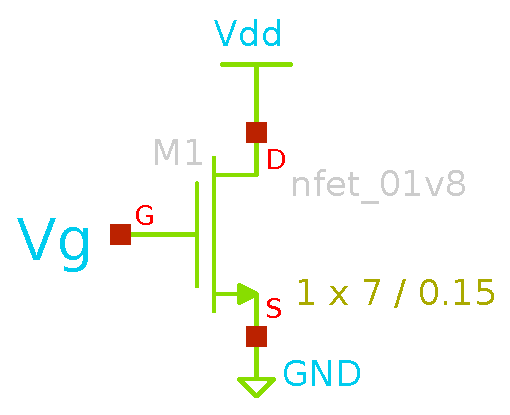
\includegraphics[width=3.3cm]{Immagini/nmos.eps}
			\caption{schematico di un transistor n-mos con bulk a massa, drain posto alla tensione di alimentazione $V_{dd}$, gate posto alla tensione $V_g$ e source a massa.} \label{fig:intro:schematico-nmos}
		\end{figure}
	
		Simulando il circuito in figura \ref{fig:intro:schematico-nmos} è possibile ottenere la caratteristica statica (figura \ref{fig:intro:nmos-carattstatica}) di trasferimento che determina la corrente $I_n$ che fluisce dal drain verso il source in funzione delle tensioni differenziali $V_{ds}$ e $V_{gs}$. Tramite questa si può anche determinare la tensione di soglia $\Vtn$ del transistor che è pari a circa $0.6V$.
		
		\begin{figure}[h!]
			\centering
			% GNUPLOT: LaTeX picture with Postscript
\begingroup
\newcommand{\ft}[0]{\footnotesize}
  \makeatletter
  \providecommand\color[2][]{%
    \GenericError{(gnuplot) \space\space\space\@spaces}{%
      Package color not loaded in conjunction with
      terminal option `colourtext'%
    }{See the gnuplot documentation for explanation.%
    }{Either use 'blacktext' in gnuplot or load the package
      color.sty in LaTeX.}%
    \renewcommand\color[2][]{}%
  }%
  \providecommand\includegraphics[2][]{%
    \GenericError{(gnuplot) \space\space\space\@spaces}{%
      Package graphicx or graphics not loaded%
    }{See the gnuplot documentation for explanation.%
    }{The gnuplot epslatex terminal needs graphicx.sty or graphics.sty.}%
    \renewcommand\includegraphics[2][]{}%
  }%
  \providecommand\rotatebox[2]{#2}%
  \@ifundefined{ifGPcolor}{%
    \newif\ifGPcolor
    \GPcolorfalse
  }{}%
  \@ifundefined{ifGPblacktext}{%
    \newif\ifGPblacktext
    \GPblacktexttrue
  }{}%
  % define a \g@addto@macro without @ in the name:
  \let\gplgaddtomacro\g@addto@macro
  % define empty templates for all commands taking text:
  \gdef\gplbacktext{}%
  \gdef\gplfronttext{}%
  \makeatother
  \ifGPblacktext
    % no textcolor at all
    \def\colorrgb#1{}%
    \def\colorgray#1{}%
  \else
    % gray or color?
    \ifGPcolor
      \def\colorrgb#1{\color[rgb]{#1}}%
      \def\colorgray#1{\color[gray]{#1}}%
      \expandafter\def\csname LTw\endcsname{\color{white}}%
      \expandafter\def\csname LTb\endcsname{\color{black}}%
      \expandafter\def\csname LTa\endcsname{\color{black}}%
      \expandafter\def\csname LT0\endcsname{\color[rgb]{1,0,0}}%
      \expandafter\def\csname LT1\endcsname{\color[rgb]{0,1,0}}%
      \expandafter\def\csname LT2\endcsname{\color[rgb]{0,0,1}}%
      \expandafter\def\csname LT3\endcsname{\color[rgb]{1,0,1}}%
      \expandafter\def\csname LT4\endcsname{\color[rgb]{0,1,1}}%
      \expandafter\def\csname LT5\endcsname{\color[rgb]{1,1,0}}%
      \expandafter\def\csname LT6\endcsname{\color[rgb]{0,0,0}}%
      \expandafter\def\csname LT7\endcsname{\color[rgb]{1,0.3,0}}%
      \expandafter\def\csname LT8\endcsname{\color[rgb]{0.5,0.5,0.5}}%
    \else
      % gray
      \def\colorrgb#1{\color{black}}%
      \def\colorgray#1{\color[gray]{#1}}%
      \expandafter\def\csname LTw\endcsname{\color{white}}%
      \expandafter\def\csname LTb\endcsname{\color{black}}%
      \expandafter\def\csname LTa\endcsname{\color{black}}%
      \expandafter\def\csname LT0\endcsname{\color{black}}%
      \expandafter\def\csname LT1\endcsname{\color{black}}%
      \expandafter\def\csname LT2\endcsname{\color{black}}%
      \expandafter\def\csname LT3\endcsname{\color{black}}%
      \expandafter\def\csname LT4\endcsname{\color{black}}%
      \expandafter\def\csname LT5\endcsname{\color{black}}%
      \expandafter\def\csname LT6\endcsname{\color{black}}%
      \expandafter\def\csname LT7\endcsname{\color{black}}%
      \expandafter\def\csname LT8\endcsname{\color{black}}%
    \fi
  \fi
    \setlength{\unitlength}{0.0500bp}%
    \ifx\gptboxheight\undefined%
      \newlength{\gptboxheight}%
      \newlength{\gptboxwidth}%
      \newsavebox{\gptboxtext}%
    \fi%
    \setlength{\fboxrule}{0.5pt}%
    \setlength{\fboxsep}{1pt}%
\begin{picture}(5668.00,3400.00)%
    \gplgaddtomacro\gplbacktext{%
      \csname LTb\endcsname%%
      \put(946,704){\makebox(0,0)[r]{\strut{}$-0.5$}}%
      \csname LTb\endcsname%%
      \put(946,979){\makebox(0,0)[r]{\strut{}$0$}}%
      \csname LTb\endcsname%%
      \put(946,1254){\makebox(0,0)[r]{\strut{}$0.5$}}%
      \csname LTb\endcsname%%
      \put(946,1529){\makebox(0,0)[r]{\strut{}$1$}}%
      \csname LTb\endcsname%%
      \put(946,1804){\makebox(0,0)[r]{\strut{}$1.5$}}%
      \csname LTb\endcsname%%
      \put(946,2079){\makebox(0,0)[r]{\strut{}$2$}}%
      \csname LTb\endcsname%%
      \put(946,2354){\makebox(0,0)[r]{\strut{}$2.5$}}%
      \csname LTb\endcsname%%
      \put(946,2629){\makebox(0,0)[r]{\strut{}$3$}}%
      \csname LTb\endcsname%%
      \put(946,2904){\makebox(0,0)[r]{\strut{}$3.5$}}%
      \csname LTb\endcsname%%
      \put(946,3179){\makebox(0,0)[r]{\strut{}$4$}}%
      \csname LTb\endcsname%%
      \put(1078,484){\makebox(0,0){\strut{}$0$}}%
      \csname LTb\endcsname%%
      \put(1544,484){\makebox(0,0){\strut{}$0.2$}}%
      \csname LTb\endcsname%%
      \put(2010,484){\makebox(0,0){\strut{}$0.4$}}%
      \csname LTb\endcsname%%
      \put(2476,484){\makebox(0,0){\strut{}$0.6$}}%
      \csname LTb\endcsname%%
      \put(2942,484){\makebox(0,0){\strut{}$0.8$}}%
      \csname LTb\endcsname%%
      \put(3407,484){\makebox(0,0){\strut{}$1$}}%
      \csname LTb\endcsname%%
      \put(3873,484){\makebox(0,0){\strut{}$1.2$}}%
      \csname LTb\endcsname%%
      \put(4339,484){\makebox(0,0){\strut{}$1.4$}}%
      \csname LTb\endcsname%%
      \put(4805,484){\makebox(0,0){\strut{}$1.6$}}%
      \csname LTb\endcsname%%
      \put(5271,484){\makebox(0,0){\strut{}$1.8$}}%
      \colorrgb{0.00,0.30,0.60}%%
      \put(3175,2904){\rotatebox{5}{\makebox(0,0){\strut{}\ft $V_{gs}=1.8V$}}}%
      \put(3175,2354){\rotatebox{4}{\makebox(0,0){\strut{}\ft $V_{gs}=1.5V$}}}%
      \put(3175,1804){\rotatebox{3}{\makebox(0,0){\strut{}\ft $V_{gs}=1.2V$}}}%
      \put(3175,1309){\rotatebox{1}{\makebox(0,0){\strut{}\ft $V_{gs}=0.9V$}}}%
      \put(3175,842){\makebox(0,0){\strut{}\ft $V_{gs}<0.8V$}}%
    }%
    \gplgaddtomacro\gplfronttext{%
      \csname LTb\endcsname%%
      \put(209,1941){\rotatebox{-270}{\makebox(0,0){\strut{}Corrente $I$ $[mA]$}}}%
      \put(3174,154){\makebox(0,0){\strut{}Tensione $V_{ds}$ $[V]$}}%
      \csname LTb\endcsname%%
      \put(3174,7828){\makebox(0,0){\strut{}}}%
    }%
    \gplbacktext
    \put(0,0){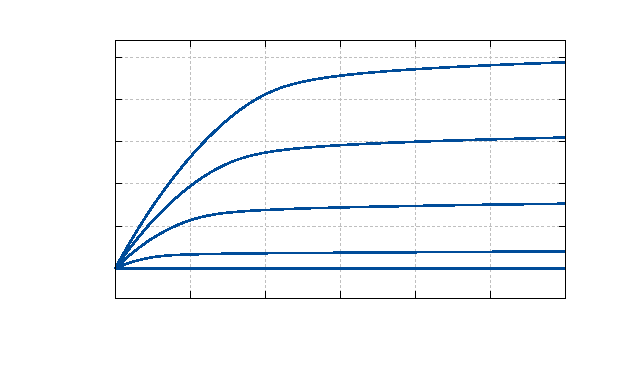
\includegraphics[width={283.40bp},height={170.00bp}]{Immagini/caratt_statica}}%
    \gplfronttext
  \end{picture}%
\endgroup

			\caption{caratteristica statica ottenuta mediante simulazione \texttt{dc sweep} del circuito in figura \ref{fig:intro:schematico-nmos}.}
			\label{fig:intro:nmos-carattstatica}
		\end{figure}
		
	
		\paragraph{Caratteristiche dinamiche} Individuate le principali caratteristiche statiche, è possibile osservare dei comportamenti dinamici del circuito legati in particolare agli andamenti dei transitori.
	
		
		\begin{figure}[bht]
			\centering
			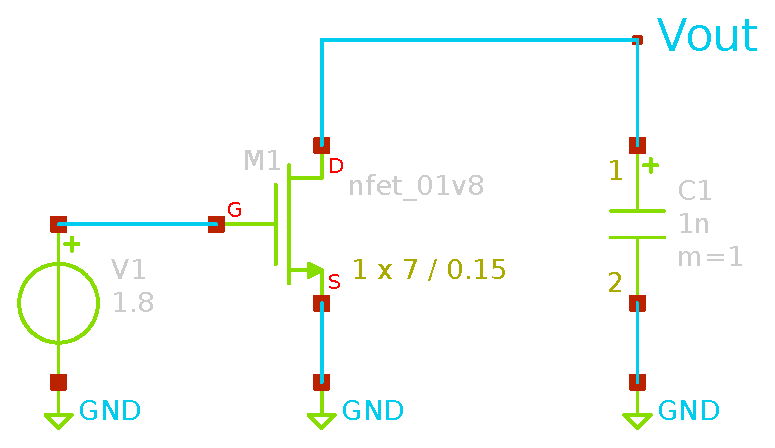
\includegraphics[width=5cm]{Immagini/circuito_transitorio.eps}
			\caption{circuito per simulare la scarica di un condensatore $C_1$ di capacità $1nF$, posto inizialmente ad una tensione $V_{out} = 1.8V$, mediante l'utilizzo di transistor n-mos.} \label{fig:intro:schematico-transitorio}
		\end{figure}
	
		Il circuito più semplice da considerare a tale fine è quello riportato in figura \ref{fig:intro:schematico-transitorio} che si basa sullo scaricare una capacità di $1nF$ mediante l'utilizzo di transistori n-mos. In questo caso si pone al massimo la tensione $\Vgs = 1.8V$ e si effettua una simulazione sul transitorio. Posto che al tempo iniziale la tensione in uscita $\Vout$ fosse pari allo stato alto $1.8V$, utilizzando i diversi modelli corner spice forniti è possibile effettuare dei diagrammi di rappresentazione dei transitori.
	
		\begin{figure}[bht]
			\centering
			% GNUPLOT: LaTeX picture with Postscript
\begingroup
  \makeatletter
  \providecommand\color[2][]{%
    \GenericError{(gnuplot) \space\space\space\@spaces}{%
      Package color not loaded in conjunction with
      terminal option `colourtext'%
    }{See the gnuplot documentation for explanation.%
    }{Either use 'blacktext' in gnuplot or load the package
      color.sty in LaTeX.}%
    \renewcommand\color[2][]{}%
  }%
  \providecommand\includegraphics[2][]{%
    \GenericError{(gnuplot) \space\space\space\@spaces}{%
      Package graphicx or graphics not loaded%
    }{See the gnuplot documentation for explanation.%
    }{The gnuplot epslatex terminal needs graphicx.sty or graphics.sty.}%
    \renewcommand\includegraphics[2][]{}%
  }%
  \providecommand\rotatebox[2]{#2}%
  \@ifundefined{ifGPcolor}{%
    \newif\ifGPcolor
    \GPcolorfalse
  }{}%
  \@ifundefined{ifGPblacktext}{%
    \newif\ifGPblacktext
    \GPblacktexttrue
  }{}%
  % define a \g@addto@macro without @ in the name:
  \let\gplgaddtomacro\g@addto@macro
  % define empty templates for all commands taking text:
  \gdef\gplbacktext{}%
  \gdef\gplfronttext{}%
  \makeatother
  \ifGPblacktext
    % no textcolor at all
    \def\colorrgb#1{}%
    \def\colorgray#1{}%
  \else
    % gray or color?
    \ifGPcolor
      \def\colorrgb#1{\color[rgb]{#1}}%
      \def\colorgray#1{\color[gray]{#1}}%
      \expandafter\def\csname LTw\endcsname{\color{white}}%
      \expandafter\def\csname LTb\endcsname{\color{black}}%
      \expandafter\def\csname LTa\endcsname{\color{black}}%
      \expandafter\def\csname LT0\endcsname{\color[rgb]{1,0,0}}%
      \expandafter\def\csname LT1\endcsname{\color[rgb]{0,1,0}}%
      \expandafter\def\csname LT2\endcsname{\color[rgb]{0,0,1}}%
      \expandafter\def\csname LT3\endcsname{\color[rgb]{1,0,1}}%
      \expandafter\def\csname LT4\endcsname{\color[rgb]{0,1,1}}%
      \expandafter\def\csname LT5\endcsname{\color[rgb]{1,1,0}}%
      \expandafter\def\csname LT6\endcsname{\color[rgb]{0,0,0}}%
      \expandafter\def\csname LT7\endcsname{\color[rgb]{1,0.3,0}}%
      \expandafter\def\csname LT8\endcsname{\color[rgb]{0.5,0.5,0.5}}%
    \else
      % gray
      \def\colorrgb#1{\color{black}}%
      \def\colorgray#1{\color[gray]{#1}}%
      \expandafter\def\csname LTw\endcsname{\color{white}}%
      \expandafter\def\csname LTb\endcsname{\color{black}}%
      \expandafter\def\csname LTa\endcsname{\color{black}}%
      \expandafter\def\csname LT0\endcsname{\color{black}}%
      \expandafter\def\csname LT1\endcsname{\color{black}}%
      \expandafter\def\csname LT2\endcsname{\color{black}}%
      \expandafter\def\csname LT3\endcsname{\color{black}}%
      \expandafter\def\csname LT4\endcsname{\color{black}}%
      \expandafter\def\csname LT5\endcsname{\color{black}}%
      \expandafter\def\csname LT6\endcsname{\color{black}}%
      \expandafter\def\csname LT7\endcsname{\color{black}}%
      \expandafter\def\csname LT8\endcsname{\color{black}}%
    \fi
  \fi
    \setlength{\unitlength}{0.0500bp}%
    \ifx\gptboxheight\undefined%
      \newlength{\gptboxheight}%
      \newlength{\gptboxwidth}%
      \newsavebox{\gptboxtext}%
    \fi%
    \setlength{\fboxrule}{0.5pt}%
    \setlength{\fboxsep}{1pt}%
\begin{picture}(5668.00,2834.00)%
    \gplgaddtomacro\gplbacktext{%
      \csname LTb\endcsname%%
      \put(814,878){\makebox(0,0)[r]{\strut{}$0$}}%
      \csname LTb\endcsname%%
      \put(814,1138){\makebox(0,0)[r]{\strut{}$0.3$}}%
      \csname LTb\endcsname%%
      \put(814,1398){\makebox(0,0)[r]{\strut{}$0.6$}}%
      \csname LTb\endcsname%%
      \put(814,1658){\makebox(0,0)[r]{\strut{}$0.9$}}%
      \csname LTb\endcsname%%
      \put(814,1919){\makebox(0,0)[r]{\strut{}$1.2$}}%
      \csname LTb\endcsname%%
      \put(814,2179){\makebox(0,0)[r]{\strut{}$1.5$}}%
      \csname LTb\endcsname%%
      \put(814,2439){\makebox(0,0)[r]{\strut{}$1.8$}}%
      \csname LTb\endcsname%%
      \put(946,484){\makebox(0,0){\strut{}$0$}}%
      \csname LTb\endcsname%%
      \put(2027,484){\makebox(0,0){\strut{}$0.5$}}%
      \csname LTb\endcsname%%
      \put(3109,484){\makebox(0,0){\strut{}$1$}}%
      \csname LTb\endcsname%%
      \put(4190,484){\makebox(0,0){\strut{}$1.5$}}%
      \csname LTb\endcsname%%
      \put(5271,484){\makebox(0,0){\strut{}$2$}}%
    }%
    \gplgaddtomacro\gplfronttext{%
      \csname LTb\endcsname%%
      \put(209,1658){\rotatebox{-270}{\makebox(0,0){\strut{} $V_{out}$ $[V]$}}}%
      \put(3108,154){\makebox(0,0){\strut{}Tempo $[n s]$}}%
      \csname LTb\endcsname%%
      \put(4284,2440){\makebox(0,0)[r]{\strut{}slow}}%
      \csname LTb\endcsname%%
      \put(4284,2220){\makebox(0,0)[r]{\strut{}typical}}%
      \csname LTb\endcsname%%
      \put(4284,2000){\makebox(0,0)[r]{\strut{}fast}}%
      \csname LTb\endcsname%%
      \put(3108,7262){\makebox(0,0){\strut{}}}%
    }%
    \gplbacktext
    \put(0,0){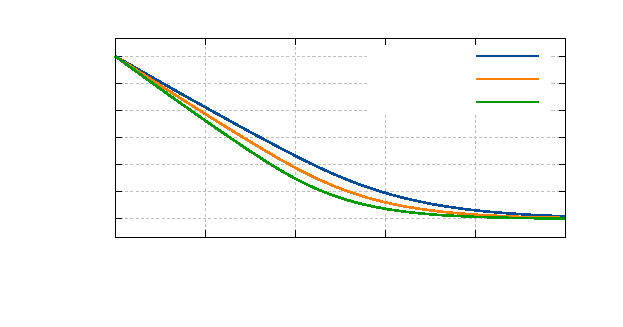
\includegraphics[width={283.40bp},height={141.70bp}]{Immagini/transitori}}%
    \gplfronttext
  \end{picture}%
\endgroup

			\caption{evoluzione della tensione in uscita $V_{out}$ dovuta alla scarica della capacità mediante un mosfet (circuito in figura \ref{fig:intro:schematico-transitorio}).}
			\label{fig:intro:nmos-tempitransitorio}
		\end{figure}
	
		Facendo riferimenti ai risultati in figura \ref{fig:intro:nmos-tempitransitorio}, è possibile osservare che modelli corner diversi, rispetto al nome loro assegnato, producono dei risultati distinti. Ipotizzando di concludere il transitorio al $90\%$ di escursione del segnale, ossia quando la tensione in uscita raggiunge il valore $V_{out} = 0.18V$, si ottengono i tempi per i 3 modelli pari a:
		\[ t_{slow} \approx 584 ns \qquad t_{typical} \approx 516 ns \qquad t_{fast} \approx 467ns    \] 
		Ove non diversamente specificato nella prosecuzione del documento tutti comportamenti transitori verranno valutati rispetto ad un comportamento tipico dei transistor.
		
	
	
	
	
	
	
	